%===================================== CHAP 5 =================================


\chapter{Solution Approach} \label{chapter_solution_approach}

In this chapter a solution approach for the FTCP is suggested. 

\section{Solution structure}
With perfect information, the model formulated in Section \ref{mathematical_model} gives the perfect team to select in each gameweek. However, the perfect information is not available until the gameweek has been played. Thus, the main uncertainty in the problem lies here. To solve for the uncertainty, a forecast of the Premier League player's expected points in a gameweek is generated. This forecast is further used as input in the optimization model which is then solved over a set of gameweek. The forecast is done in such way that recent performance is weighted according to a weighting function, and updated whenever a gameweek is played. By such one captures the dynamic development of team's and player's performances, and thus taking account for which players are in good form. Recent form plays an important role when managers make their FPL decisions, and is considered as an important indicator for future performance.   

\newpar
\newpage
When using a forecast to estimate the expected value of a player's points, the objective function described in Section \ref{mathematical_model} changes from: 

\begin{equation*}
\text{max} \; z = \EX_{\omega} \Big\lbrack\sum_{p \in \mathcal{P}} \sum_{t \in \mathcal{T}} \Big( \mathlarger{\rho}_{pt}(\omega)y_{pt} +  \mathlarger{\rho}_{pt}(\omega)f_{pt} + \epsilon \mathlarger{\rho}_{pt}(\omega)h_{pt} + \sum_{l \in \mathcal{L}}\sigma_{l} \mathlarger{\rho}_{pt}(\omega)g_{ptl} \Big) \Big\rbrack - R\sum_{t \in \mathcal{T}}\alpha_{t}
\end{equation*}

to 

\begin{equation*}
\text{max} \; z = \sum_{p \in \mathcal{P}} \sum_{t \in \mathcal{T}} \Big( \hat{\mathlarger{\rho}}_{pt} y_{pt} + \hat{\mathlarger{\rho}}_{pt}f_{pt} + \epsilon \hat{\mathlarger{\rho}}_{pt}h_{pt} + \sum_{l \in \mathcal{L}}\sigma_{l} \hat{\mathlarger{\rho}}_{pt} g_{ptl} \Big) - R\sum_{t \in \mathcal{T}}\alpha_{t}
\end{equation*}

where $\hat{\rho}_{pt}$ denotes the expected points of each player $p$ in a gameweek $t$.

\newpar

NOTE:TA MED 6.2.2 Test Method FRA PROSJEKTET. JUSTERT. SKRIVE FOR HVORDAN VALGENE FOR CHIP BLUR JUSTERT FOR MELLOM HORISONTENE.


\section{Player performance prediction}
The optimization model presented in chapter \ref{model_formulation} uses expected fantasy points as an input. A major uncertainty lies in prediction of football players performances. In this section, we introduce three different methods of predicting future player performance. First, we present a regression model based on the historical Fantasy Premier League performance. Secondly, we replicate and modify the approach suggested by \cite{Bonomo}. Finally, we introduce an approach using bookmakers odds' in order to predict each players expected points. 

\subsection{Player prediction using regression}

\subsubsection{Theory}

One way of predicting Fantasy Premier League points is by use of regression. By running a regression model, one can figure out which data that is most related to a player's performance. For instance, it is interesting to see how a player's achieved points are related to the opponent he is facing, as well as how his position on the field is relevant for the amount of points he receives. This can be done for numerous factors influencing the outcome of a football match. Some of the factors are predetermined and available for the managers throughout the season, while others may vary during the season. In the following, some interesting regression variables are presented: 
\newpar
\textit{Stochastic factors influencing FPL points:}
\newpar
\begin{itemize}
    \item A \textbf{realized points} variable can be used as the dependent variable as which the other variables are measured towards. The realized points are the actual points gained by a player for previous gameweeks.
    \item Variables for \textbf{previous matches} are incorporated in order to check whether recent performance influence the actual performance of upcoming gameweeks.
    \item It is reasonable to assume that a player who plays for a good \textbf{team} is expected to gain many points as his team performs well. For instance, defenders playing for teams that does not concede many goals are most likely to keep a clean sheet.
    \item The \textbf{cost} of a player gives an impression of the quality of that particular player. A player listed with a high cost, is expected to gain many points during the season. It would therefore be interesting to check the correlation between a player's cost and his actual point performance. 
    \item \textbf{Transfers} made by FPL managers gives one an impression of how other managers expect a player to perform in the future.
    \end{itemize}
\newpar
\textit{Deterministic factors influencing FPL points}
\newpar
\begin{itemize}
    \item The \textbf{position on the field} is worth some attention as well. For instance, it would be interesting to check whether midfielders gain more points than defenders. By figuring out which positions one should focus on, it might be optimal to find an optimal formation for a FPL team.
    \item An important factor is the \textbf{opponent team} a team is facing for a particular gameweek. It is likely that a player gain more points against a rather poor team than a top-ranked team. 
\end{itemize}





\subsection{Average performance prediction}
\subsubsection{Theory}
The solution approach suggested by \cite{Bonomo} can be used for the English Fantasy Premier League as well as for the Argentinian. In general, one simply use the average points performance for the recent gameweeks as the prediction of the performance for the next gameweek. In order to improve the prediction, one can account for team opponent, home advantage and whether a player is on a good performance streak. This is done by weighting a player's performance by three factors as mentioned in section \ref{Forecasting_of_player_performance}.
\newpar
In general, a player's point prediction is calculated according to the following equation:
\begin{equation}
    \textrm{Expected points} = \textrm{Adjusted avg. points} \times \textrm{Team strength} \times \textrm{Home advantage} \times \textrm{Point streak}
\end{equation}
\newpar
Firstly, the solution approach suggested by \cite{Bonomo} is replicated for Fantasy Premier League using their recommended numerical values. Next, we intend to modify and improve the model by using different weights adjusted for historical performance in the English Premier League. Instead of weighting the teams based on their league position, we utilize an Elo-rating in order to weight the relative team strengths in the league. In addition, an empirical value of home field advantage in the Premier League is used as a factor for the home advantage. In order to measure a player's recent performance, decisions are made on whether a player is on a positive or negative point streak. 
\subsubsection{The Elo system}

The Elo system introduced in section \ref{Strength_of_football_teams} is a rating system used for measuring the relative strength level of sport teams and individual athletes. Within football, the Elo system can be used in order to determine a club's Elo value. The great advantage of the Elo system lies in its simplicity, there is only one value per club at each point in time, the higher the better. 
\newpar
The performance of a team is not measured absolutely; it's inferred from wins, losses and draws against other teams. If team A has a Elo value of $R_A$ and team B has a Elo value of $R_B$, team A has an expected score of 
\begin{equation}\label{eq5.2}
    E_A = \frac{1}{1+10^{\frac{R_B - R_A}{400}}}
\end{equation}
when facing team B. Similarly, team B has an expected score of
\begin{equation}\label{eq5.3}
    E_B = \frac{1}{1+10^{\frac{R_A - R_B}{400}}}
\end{equation}

\newpar
When teams play each other and win or lose, they exchange points. Hence, the club's Elo value is updated once a match has been played. Using the expected scores from equation \ref{eq5.2}, team A's updated Elo value is calculated according to
\begin{equation} \label{eq5.4}
    R^{'}_A = R_A + (S_A-E_A) \times k
\end{equation}
where $S_A$ is the result (1 for win, 0.5 for draw and 0 for loss). Further, $k$ is a factor which determines how fast the Elo value will converge. A higher k-value will have the values converging quicker to their true values, but will suffer from more variation. For smaller k-values, more stable Elo values are created which take longer time to converge. In chess, the World Chess Federation suggest that a value of k=20 should be used for players with an Elo value below 2400. 
\newpar
Similarly, team B's updated Elo value is given by
\begin{equation} \label{eq5.5}
    R^{'}_B = R_B + (S_B-E_B) \times k
\end{equation}
\newpar
In the following, an illustrating example provide how the Elo value of two teams are updated once a match between them has been played:
\newpar
Assume that team A has an Elo value of 1881 and that team B has a value of 1650. If team A faces team B, team A has an expected score according to equation \ref{eq5.2}:
\begin{equation*}
    E_A = \frac{1}{1+10^{\frac{1650-1881}{400}}} = 0.791
\end{equation*}
while team B has an expected score of
\begin{equation*}
    E_B = \frac{1}{1+10^{\frac{1881-1650}{400}}} = 0.209
\end{equation*}
Further, if team A won the match, its Elo value will increase to a value according to equation \ref{eq5.4}: 
\begin{equation*}
   R^{'}_A= 1881 + (1-0.791) \times 20 = 1885
\end{equation*}
As for team B, its Elo value decreases to
\begin{equation*}
   R^{'}_B = 1650 + (0-0.209) \times 20 = 1646 
\end{equation*}

\subsubsection{Using Elo values to rate Premier League teams}
The Elo values provide a sophisticated measurement of the relative strength between the Premier League teams. Further, as the values are updated once a match has been played, the Elo system somehow catches which teams that are in a good form. Elo values can be obtained according to equation \ref{eq5.1} and \ref{eq5.2}. Clubelo.com provide historical Elo values for most of the professional football teams in the world, including teams in the English Premier League, English 1st division etc. These values are used in order to compute the relative team strength in this project, using a k-value of 20. A great advantage of the ratings provided by Clubelo is the fact that these values are modified, taking account for home field advantage, goal difference and inter-league adjustments. In addition, the Elo values from Clubelo incorporates all fixtures and not only league matches.
\newpar
Once the Elo values are obtained, they can be used in order to weight the previous performance of each Fantasy Premier League player. It is likely to suggest that a player playing for a top-rated team has a greater probability of scoring many points than a player playing for a poor team. In addition, a player is more likely to gain many points against a weak opponent than against a top-rated team. Hence, one should consider both the opponent and the team of a player when calculating his previous average. 
\newpar
In table \ref{Elo.1617} some Elo values for the first gameweeks of the English Premier League 2016/17 season are listed. Note that the values are calculated ahead of each gameweek, so that the values in the GW1 column are the Elo values of the teams before gameweek 1 has been played. 

\begin{table}[H]
\centering
\caption{Elo ratings for Premier League 2016/2017}
\label{Elo.1617}
\begin{tabular}{|l|l|l|l|l|l|}
\cline{2-6}
\multicolumn{1}{l|}{} & \multicolumn{1}{l|}{} & \multicolumn{4}{c|}{Elo value}  \\ \cline{2-6} 
\hline
                      & Team                  & GW1    & GW2    & GW3  & GW4    \\
                      \hline
1                     & Chelsea               & 1793   & 1800   & 1798 & 1804   \\
2                     & Tottenham             & 1804   & 1804   & 1800 & 1798   \\
3                     & Man City              & 1848   & 1856   & 1858 & 1863   \\
4                     & Man Utd               & 1789   & 1797   & 1799 & 1804   \\
-                     &                       &        &        &      &        \\
-                     &                       &        &        &      &        \\
-                     &                       &        &        &      &        \\
17                    & Watford               & 1624   & 1631   & 1618 & 1612   \\
18                    & Hull                  & 1589   & 1603   & 1613 & 1608   \\
19                    & Middlesbrough         & 1595   & 1597   & 1601 & 1604   \\
20                    & Sunderland            & 1655   & 1654   & 1636 & 1641   \\
\hline
\end{tabular}
\end{table}

Values from table \ref{Elo.1617} can be used in order to weight the performance of a player. For instance, if a forward received many points against Chelsea, that is more impressive than if the same player equally many points against Sunderland. Hence, one should weight the performances appropriately. In the following, an approach for weighting historical performance is suggested. For instance, let's assume that Paul Pogba, a midfielder at Manchester United received the following points for the first three gameweeks: 


\begin{table}[H]
\centering
\caption{Paul Pogba imaginary points}
\label{my-label}
\begin{tabular}{|l|l|l|l|l|}
\hline
\multicolumn{1}{|c|}{} & \multicolumn{4}{c|}{Points Gained} \\ \hline
Opponent               & GW1        & GW2       & GW3    & GW4   \\
\hline
Chelsea                & 6          &           &        &       \\
Sunderland             &            & 9         &        &       \\
Watford                &            &           & 10     &         \\
Tottenham              &            &           &        & ?      \\
\hline
\end{tabular}
\end{table}

If one simply used his average score for the past three gameweeks in order to predict his performance for the next gameweek, one would predict Pogba to gain 8.33 points in gameweek 4. However, in this case one do not take account for the fact that Manchester United were facing teams of different quality. In addition, one does not consider the fact that Pogba plays for Manchester United, a team that in general performs better than most other teams. As mentioned above, these factors should be considered. Hence, it is necessary to weight the previous performance taking account for the opponent team and the player's team. This can be solved in the following way: 
\newpar
In gameweek 1, Manchester United were facing Chelsea and Pogba earned 6 points. In order to take account for the fact that Pogba plays for Manchester United and were facing Chelsea (a higher ranked team), one simply mulitply his score with Chelseas Elo value and divide it by Manchester Uniteds Elo value. Thus, Paul Pogbas adjusted points should be set to:
\begin{equation*}
    \textrm{Paul Pogba GW1} = 6 \times \frac{1793}{1789} = 6.013 
\end{equation*}
As can be observed, his actual points increases when facing an opponent that is assumed to be better than his team. In contrary, when facing a weaker team, for instance Sunderland his realistic points decreases: 
\begin{equation*}
    \textrm{Paul Pogba GW2} = 9 \times \frac{1654}{1797} = 8.284 
\end{equation*}

In general a players realistic points gained can be calculated by the following equation: 
\begin{equation} \label{actualpoints}
\textrm{Realistic points} = \textrm{Adjusted points} \times \frac{\textrm{Opponent Elo value}}{\textrm{Player's team Elo value}}    
\end{equation}

By calculating realistic points according to equation \ref{actualpoints}, Paul Pogbas adjusted average for the first three gameweeks would be 7.764. The following equation is used in order to calculate the expected points for an upcoming gameweek: 
\begin{equation}
    \textrm{Expected points} = \textrm{Adjusted average} \times \frac{\textrm{Player's team Elo value}}{\textrm{Opponent Elo value}}
\end{equation}
In this way, players are rewarded with an increased expected points when playing for a team with a higher Elo value than its opponent. Hence, his expected performance against Tottenham in the upcoming gameweek 4 would be: 
\begin{equation*}
    \textrm{Expected points for Pogba GW4} = 7.764 \times \frac{1804}{1798} = 7.790
\end{equation*}


\subsubsection{Home field advantage}
As pointed out in section \ref{HomeFieldAdvantage} numerous studies have proven that some kind of home field advantage exist when football games are being played. Football teams have a tendency of performing better when playing at their home field then when playing at their opponents ground. This home field advantage has to be considered when one are to forecast the upcoming performance of the Premier League players. 
\newpar
Usually when one is to determine the home field advantage in a football league, one focuses on the outcome of the game, i.e.  win, draw or loss. In Fantasy Premier League, the outcome of a match has no impact in the point system. As the most important point-factor in FPL is goals scored, the home field advantage has to be calculated in terms of goals. 
\newpar
The home field advantage can be calculated according to the approach suggested by \cite{Pollard}. However, instead of focusing of match outcomes, one determine the advantage by looking into goals. Imagine that each team plays 38 matches during the season, equally divided between home and away games. With 20 teams facing each other twice a season, that implies a total of 380 matches a season. Further, assume that a total of 1000 goals were scored during a particular season. If there were no home field advantage, one would expect that 500 of the goals were scored by the home team and 500 by the away team, yielding a factor of 0.5. However, the results show that 620 of the goals were scored by the home team, which represents 62 \% of the goals scored. With an expected value of 50 \% and an actual value of 62 \% the home field advantage in terms of goals scored can be calculated by: 
\begin{equation*}
    \textrm{Home field advantage} = \frac{\textrm{Actual goals scored home}}{\textrm{Expected goals scored away}} = \frac{0.62}{0.5} = 1.24 
\end{equation*}

Similarly, the away field advantage is calculated according to:
\begin{equation*}
    \textrm{Away field advantage} = \frac{\textrm{Actual goals scored away}}{\textrm{Expected goals scored away}} = \frac{0.38}{0.5} = 0.76
\end{equation*}
\newpar
In this thesis the home field advantage is calculated as an empirical value for the entire Premier League. Hence, each team's home field advantage is not considered. The idea is that the empirical home field advantage along with the relative team strengths calculated by use of the Elo system will give an appropriate representation of a team's performance both home and away. 
\newpar
In order to find an appropriate empirical value for the home field advantage, several previous seasons should be considered. In this project thesis, the empirical value is set to the average of the home field advantage over the past five Premier League seasons. This is due to the fact that the home field advantage value has been stabilized over the past seasons. 

\subsubsection{Player point streak}
Fantasy Premier League managers have a tendency of selecting players that are on a great point streak. As mentioned in section \ref{Forecasting_of_player_performance} \cite{Bonomo} add a factor in order to take account for players point streak. This factor can take a value between 0.95 and 1.05, depending on the duration of a player's point streak. Unfortunately, they do not describe how they determine the value of the point streak factor. Intuitively, the point streak value can be determined in the following way: 
\newpar
If a player receives more than X points 2 gameweeks in a row, his point streak value will be set to 1.01. Further, if the streak continues, the value will increase by 0.01 for each match that his points exceed the X number of points. When a player has received more than X points 6 gameweeks in a row, his point streak value is set to the maximum of 1.05. Hence, the value does not increase if his streak exceeds 6 matches. The same rule applies for players scoring less than Y points 2 gameweeks in a row; then his streak value will be set to 0.99. When scoring less than Y points 6 matches in a row, the point streak value is set to a minimum of 0.95. Once the scoring streak is broken, the player's value is set to 1. 




\subsection{Prediction using odds}
\subsubsection{Theory}
A quite different approach for player point prediction is by use of odds created by bookmakers. It is reasonable to assume that bookmakers provide a realistic odds distribution for the different scorelines, in order to avoid gamblers profiting from an incorrectly odds. By acquiring the result outcomes for each Premier League match, a scoreline prediction can be obtained. By summing all the result odds and dividing each individual result odds by that sum, one can obtain the probability of an exact result to occur. A great drawback with this approach, is the fact that bookmakers only provide odds for the upcoming gameweek. Hence, the odds can only be used in order to predict the fantasy points one gameweek ahead. 
\newpar
When the scoreline predictions are acquired by use of result odds, one has to link these predictions to player performances. In order to determine the probability for a defender or midfielder to keep a clean sheet, one simply sum the probabilities of each match outcome where its team does not concede a goal. Further, bookmakers provide odds' for each individual player to score a goal or have an assist in a particular match. By summing the goalscorers odds, one can obtain the cumulative probability distribution of the goalscorers. Once the cumulative distribution is obtained, one simply multiply the goalscoring probabilities with the result probabilities in order to assign goalscoring points for each player. As for the assist, a similar approach may be used. However, some of the goals scored are unassisted which must be taken account for when predicting the assist points. This can be done by multiplying a players assist points with a factor representing the amount of goals being assisted. Finally, as for the yellow cards, one simply use the odds in order to calculate the probability of a player receiving a yellow card. For instance, if a player has a probability of 0.3 for receiving a yellow card in a particular match, his expected points is penalized with -0.3 as a yellow card deducts 1 point. 
\newpar
The largest bookmaking companies offers odds for all the items mentioned in the paragraph above. As goals scored are the greatest point factor in Fantasy Premier League, this area is of great interest. As mentioned, it is necessary to to obtain the probabilities for each result outcome in a given match. The following example provides Unibet's result odds for a match-up between Leicester and Burnley on April 14th 2018. 

\begin{table}[H]
\centering
\caption{Result odds for Leicester-Burnley 14.04.18}
\label{Leicester-Burnley}
\begin{tabular}{|ll|ll|ll|}
\multicolumn{6}{c}{Odds}                   \\
\hline
1-0 & 7.00   & 0-0 & 7.50   & 0-1 & 8.00   \\
2-0 & 11.00  & 1-1 & 6.00   & 0-2 & 13.00  \\
2-1 & 9.50   & 2-2 & 15.00  & 1-2 & 10.50  \\
3-0 & 23.00  & 3-3 & 67.00  & 0-3 & 29.00  \\
3-1 & 21.00  & 4-4 & 301.00 & 1-3 & 23.00  \\
3-2 & 31.00  &     &        & 2-3 & 35.00  \\
4-0 & 61.00  &     &        & 0-4 & 81.00  \\
4-1 & 56.00  &     &        & 1-4 & 67.00  \\
4-2 & 81.00  &     &        & 2-4 & 91.00  \\
4-3 & 181.00 &     &        & 3-4 & 201.00 \\
5-0 & 201.00 &     &        & 0-5 & 276.00 \\
5-1 & 181.00 &     &        & 1-5 & 226.00 \\
5-2 & 276.00 &     &        &     &        \\
\hline
\end{tabular}
\end{table}

The odds provided in table \ref{Leicester-Burnley} can be translated into match result probabilities. This is done by summing all the inverse odds and afterwards dividing each inverse odds by the sum. The results are shown in table \ref{Prob.Lei-Bur}.


\begin{table}[H]
\centering
\caption{Probabilities for Leicester-Burnley 14.04.18}
\label{Prob.Lei-Bur}
\begin{tabular}{|ll|ll|ll|}
\multicolumn{6}{c}{Odds}                         \\
\hline
1-0 & 0.104388 & 0-0 & 0.097429 & 0-1 & 0.09134  \\
2-0 & 0.066429 & 1-1 & 0.121786 & 0-2 & 0.056209 \\
2-1 & 0.076918 & 2-2 & 0.048714 & 1-2 & 0.069592 \\
3-0 & 0.03177  & 3-3 & 0.010906 & 0-3 & 0.025197 \\
3-1 & 0.034796 & 4-4 & 0.002428 & 1-3 & 0.03177  \\
3-2 & 0.023571 &     &          & 2-3 & 0.020878 \\
4-0 & 0.011979 &     &          & 0-4 & 0.009021 \\
4-1 & 0.013049 &     &          & 1-4 & 0.010906 \\
4-2 & 0.009021 &     &          & 2-4 & 0.00803  \\
4-3 & 0.004037 &     &          & 3-4 & 0.003635 \\
5-0 & 0.003635 &     &          & 0-5 & 0.002648 \\
5-1 & 0.004037 &     &          & 1-5 & 0.003233 \\
5-2 & 0.002648 &     &          &     &         \\
\hline
\end{tabular}
\end{table}

Once these probabilities are obtained, it is possible to calculate the expected goals scored by Leicester. This is done by multiplying the probability of a result occuring by the amount of goals scored by Leicester in that particular result. Further, one have to sum all the probabilities in order to find Leicester's expected goals scored. In the example from table \ref{Prob.Lei-Bur} Leicester's expected goals is found to be 1.234. 
\newpar
Further, it is necessary to assign expected goalscoring- and assist points to each player. For instance, if Jamie Vardy has a cumulative probability of 0.26 of scoring a goal for Leicester, his expected goalscoring odds is found by multiplying 0.26 with the expected goals scored by Leicester. 
\begin{equation*}
    \textrm{Jamie Vardy expected goals scored} = 1.234 \times 0.26 = 0.321
\end{equation*}

Finally, his expected points gained from scoring goals is calculated according to the Fantasy Premier League point system: 

\begin{equation*}
    \textrm{Goal points Jamie Vardy} = 0.321 \times \textrm{4 points} = \textrm{1.284 points}
\end{equation*}

A similar approach can be used in order to calculate a player's expected points from assists. However, one have to consider the fact that not all goals are assisted: 

\begin{equation*}
    \textrm{Expected assist points} = \textrm{Expected goals} \times \textrm{Player's assist probability} \times \textrm{Assist probability}
\end{equation*}

As for the clean sheets, the probability of a team keeping a clean sheet is found by summing the probabilities of all the result outcomes were the team does not concede a goal. According to table \ref{Prob.Lei-Bur} Leicester has got a probability of 0.316 for keeping a clean sheet. Hence, the starting defenders and the  goalkeeper are expected to gain

\begin{equation*}
    0.316 \times \textrm{4 points} = \textrm{1.264 points}
\end{equation*}
from keeping a clean sheet. 

\newpar
In addition, one can use odds for yellow cards in order to calculate a player's expected deducted points for receiving a yellow card. On the bookings sites each player is listed with an odds for a probability of being booked. The probability of receiving a yellow card is simply the inverse of the odds. For instance, if a player is listed with an odds of 3.00 for receiving a yellow card, it is a probability of

\begin{equation*}
    \frac{1}{3.00} = 0.333 
\end{equation*}

that the player receives a yellow card. Hence, his expected points is deducted with:

\begin{equation*}
    0.333 \times \textrm{1 point} = \textrm{0.333 points.} 
\end{equation*}

\subsubsection{Experimental setup}
As it is quite time consuming to gather all the necessary odds in order to calculate expected fantasy points, this approach requires either great computational skills. One way of solving this is by scrapping the bookmaker's website in order to obtain all the odds. Further, one have to translate all the odds into probabilities of different events to occur. 
\newpar
In order to obtain necessary data, we have cooperated with Sportradar, a Norwegian company providing data for bookmakers. Sportradar delivers odds and probabilities of several sports events, including English Premier League. They have provided us with all the necessary probabilities, including result outcomes for each Premier League match as well as individual player probabilities. These data made all the computational work a lot easier, as Sportradar exported excel files containing all the necessary data. 
\newpar
Kanskje skrive noe om format og behandling av dataen. Dette gjøres når all data fra Sportradar er på plass...

\section{Expected Value/Variance trade-off}

In financial optimization it is common to examine the expected return/variance trade-off (Markowitz). According to Zenios, the variance of a portfolio of \textit{n} assets with weight \textit{w} can be expressed as 

\begin{equation}
    \sigma^2(w) = \sum_{i = 1}^{n}\sum_{i' = 1}^{m}\sigma_{ii'}w_iw_{i'} = \sum_{i = 1}^{n}\sigma_{i}^2w_i^2 + \sum_{i = 1}^{n}\sum_{\substack{i' = 1;\\ i' \neq i}}^{n}\sigma_{ii'}w_iw_{i'}
    \label{eq:port_var}
\end{equation}

where, $w_i$ is the portfolio weight of asset $i$, $\sigma_{i}^2$ is the variance of asset \textit{i} and $\sigma_{ii'}$ is the covariance between assets $i$ and $j$. \newpar

In our case, we can rewrite Equation \ref{eq:port_var} by utilizing the fact that each portfolio weight is either $\frac{1}{11}$ or $0$. If we also substitute the expression for covariance with correlation, the expression simplifies to

\begin{equation}
    \sigma^2(y) = (\frac{1}{11})^2\sum_{i = 1}^{n}\sigma_i^2y_i + (\frac{1}{11})^2\sum_{i = 1}^{n}\sum_{\substack{i' = 1;\\ i' \neq i}}^{n} \sigma_i^2\sigma_j^2y_iy_j\rho_{i,j}
    \label{eq:team_var}
\end{equation}

where $\sigma_{i}^2$ is the variance of asset \textit{i}, $\sigma_{j}^2$ is the variance of asset \textit{j} and $\rho_{i,j}$ is the correlation between asset $i$ and asset $j$. In addition, $y_i$ and $y_j$ are binary variables indicating whether player $i$ and player $j$ is included in the starting team (portfolio) of players.\newline

In the optimization, we now may determine an upper threshold for the variance of the team at time $t$ as described below. Note that in Equation \ref{eq:team_var} two binary variables are multiplied. In order to linearize the expression, the following set of equations are inferred.

\begin{equation}
    \sigma^2_{t} = (\frac{1}{11})^2\sum_{p = 1}^{P}\sigma_p^2 y_{pt} + (\frac{1}{11})^2\sum_{p = 1}^{P}\sum_{p' = 1}^{P} \sigma_p^2\sigma_p'^2\rho_{p,p',t} \delta_{pp't} \qquad\qquad t \in \mathcal{T}
\end{equation}

\begin{equation}
    \sigma^2_{t} \leq THRESHOLD \qquad\qquad t \in \mathcal{T}
\end{equation}

\begin{equation}
    \delta_{pp't} \leq y_{pt}  \qquad\qquad p \in \mathcal{P}, p' \in \mathcal{P}, \enskip t \in \mathcal{T}
\end{equation}

\begin{equation}
    \delta_{pp't} \leq y_{p't}  \qquad\qquad p \in \mathcal{P}, p' \in \mathcal{P}, \enskip t \in \mathcal{T}
\end{equation}

\begin{equation}
    \delta_{pp't} \geq y_{pt} + y_{p't} - 1  \qquad\qquad p \in \mathcal{P}, p' \in \mathcal{P}, \enskip t \in \mathcal{T}
\end{equation}


\subsection{Variance estimation}
By variance, the variability in each players performance (points obtained) is meant. Some midfielders are known to be consistently starting, but seldom contribute in terms of assists or goals. Such players probably have a low expected value of points, but also a low variability in points earned. Other players might contribute a lot in terms of assists and goals when they are playing, but are perhaps often injured. Such players could have a high predicted value, but also a high variance in points obtained.\newpar

In order to estimate the variance of each player, their historical performance is considered. The variance is calculated as the empirical variance in points obtained for each individual player. All previous available data from the 2016/2017 and the 2017/2018 season are used. That is, for gameweek 10 of the 2017/2018, data from all rounds of the 2016/2017 as well as the first nine round of the 2017/2018 season is used.\newpar

\subsubsection{Special cases}
\textit{Lack of historical data}\newline
As mentioned in ... data for the 2016/2017 season is not available for all players. If only one data point is available for a player (i.e he has only played one match), it is impossible to calculate his variance. In these cases, the variance is set equal to the average variance of all other players. (Mention that this is only problematic in 1 round, at least for average/regression?). The lack of data points are obviously a limitation of the accuracy of the variance estimation, and constitutes a significant weakness of the method. As the variance trade-off is considered a mean to reduce overall risk, another approach/improvement might consider only picking players with a history of say 10 matches. \newpar

\textit{Zero Variance}\newline
Some players have never played, but can be selected. These players might be interesting to choose for instance to fulfill the budget/number of players constraints. However, their empirical variance would equal 0. This is not desirable, as the future performance is not deterministic (they are \textit{not} analogous the the risk-free asset in a portfolio optimization setting). Therefore, their variance is set equal the lowest non-zero variance obtained by other players.

\subsection{Correlation Estimation}
The variance of each player only considers each player's individual contribution to the team's total variance. However, it is natural to assume that there exists a correlation between the performance of players. For instance, as both a goalkeeper and defenders of the same team points for keeping a clean sheet, their performances are expected to be positively correlated. Similarly, it is intuitive that the goalkeeper and forwards of two opposing teams are negatively correlated. Whether or not there exists correlation between defenders of opposing teams are perhaps not so obvious. \newpar

In order to determine the correlation between two players on the same or opposing teams, historical data for the 2016/2017 season is considered. Note that data is aggregated such that only the correlation coefficient between different positions overall is considered. It is not calculated between individual players or teams. Therefore, the correlation between players in the same position in the same team is set equal to 1. In order to determine if a correlation coefficient is significantly different from 0, a hypothesis test is performed. The correlation between players that are not on the same team, nor facing each other in a game-week, is assumed to be 0.\newpar

Table \ref{tab:cor_team} and Table \ref{tab:cor_opp} show the correlation coefficient between different positions as well as the p-value from a hypothesis test with alternative hypothesis of a correlation not equal to 0, for players of the same and opposing teams respectively. In the cases where the correlation is not significant (GLK FWD and DEF FWD of the same teams and GLK GLK of opposing teams), the correlation coefficient is set equal to 0.

\begin{table}[H]
\centering
\caption{Correlation coefficient and p-value from significance test for the correlation between players of the same team}
\label{tab:cor_team}
\begin{tabular}{llll}
Position & Position & $\rho$    & p-value  \\
GLK      & DEF      & 0.689  & 2.20 E-16 \\
GLK      & MID      & 0.274  & 1.24 E-10 \\
GLK      & FWD      & 0.0288 & 0.519    \\
DEF      & MID      & 0.368  & 2.20 E-16 \\
DEF      & FWD      & 0.0578 & 0.176    \\
MID      & FWD      & 0.238  & 1.72 E-08
\end{tabular}
\end{table}

\begin{table}[H]
\centering
\caption{Correlation coefficient and p-value from significance test for the correlation between players of opposing teams}
\label{tab:cor_opp}
\begin{tabular}{llll}
Position & Position & $\rho$    & p-value  \\
GLK      & GLK      & 0.0162 & 0.759    \\
GLK      & DEF      & -0.106 & 0.0374   \\
GLK      & MID      & -0.312 & 2.78E-10 \\
GLK      & FWD      & -0.336 & 3.85E-16 \\
DEF      & DEF      & -0.319 & 2.35E-11 \\
DEF      & MID      & -0.447 & 2.20E-16 \\
DEF      & FWD      & -0.292 & 3.35E-09 \\
MID      & MID      & -0.254 & 1.00E-07 \\
MID      & FWD      & -0.136 & 0.00632 \\
FWD      & FWD      & -0.119 & 0.0218  
\end{tabular}
\end{table}

\subsection{Further discussion}
\begin{itemize}
    \item Na = average (bare aktuelt når spilleren kun har spilt en kamp, før det vil han ikke velges) 
    \item 0 = min $>$ 0
    \item tar med alle tilgjengelige observasjoner
    \item diskutere om fordeling
    \item varians eller standardavvik
    \item only non-zero data considered
    \item what hypotesis test is performed
\end{itemize}

\section{Determining optimal forecasting horizon, optimization horizon and penalty term for the average base method}

In a case with perfect information available, the optimal optimization horizon is the complete season of 38 weeks. Furthermore, the penalty term would be 4, equal as in the real case. However, we do not operate within the domain of perfect information, so these parameter settings are not guaranteed optimal. In addition, it is important to decide how many matches to look back in the past when calculating the forecasts based on average performance in previous games.\newpar 

In order to set the values of the parameters in a smart way, a number of different combinations of the three parameters are run on the 2016/2017 season. Figure \ref{fig:pen_hor_scale} displays how the mean value of points for the entire 2016/2017 season changes with different forecasting horizons, optimization horizons and penalty terms. Based on the figure, a combination found in the upper leftmost corner appears to be optimal, and the values $h = 2$ and $p = 18$ are chosen.

\begin{figure}
\label{fig:pen_hor_scale}
    \centering
    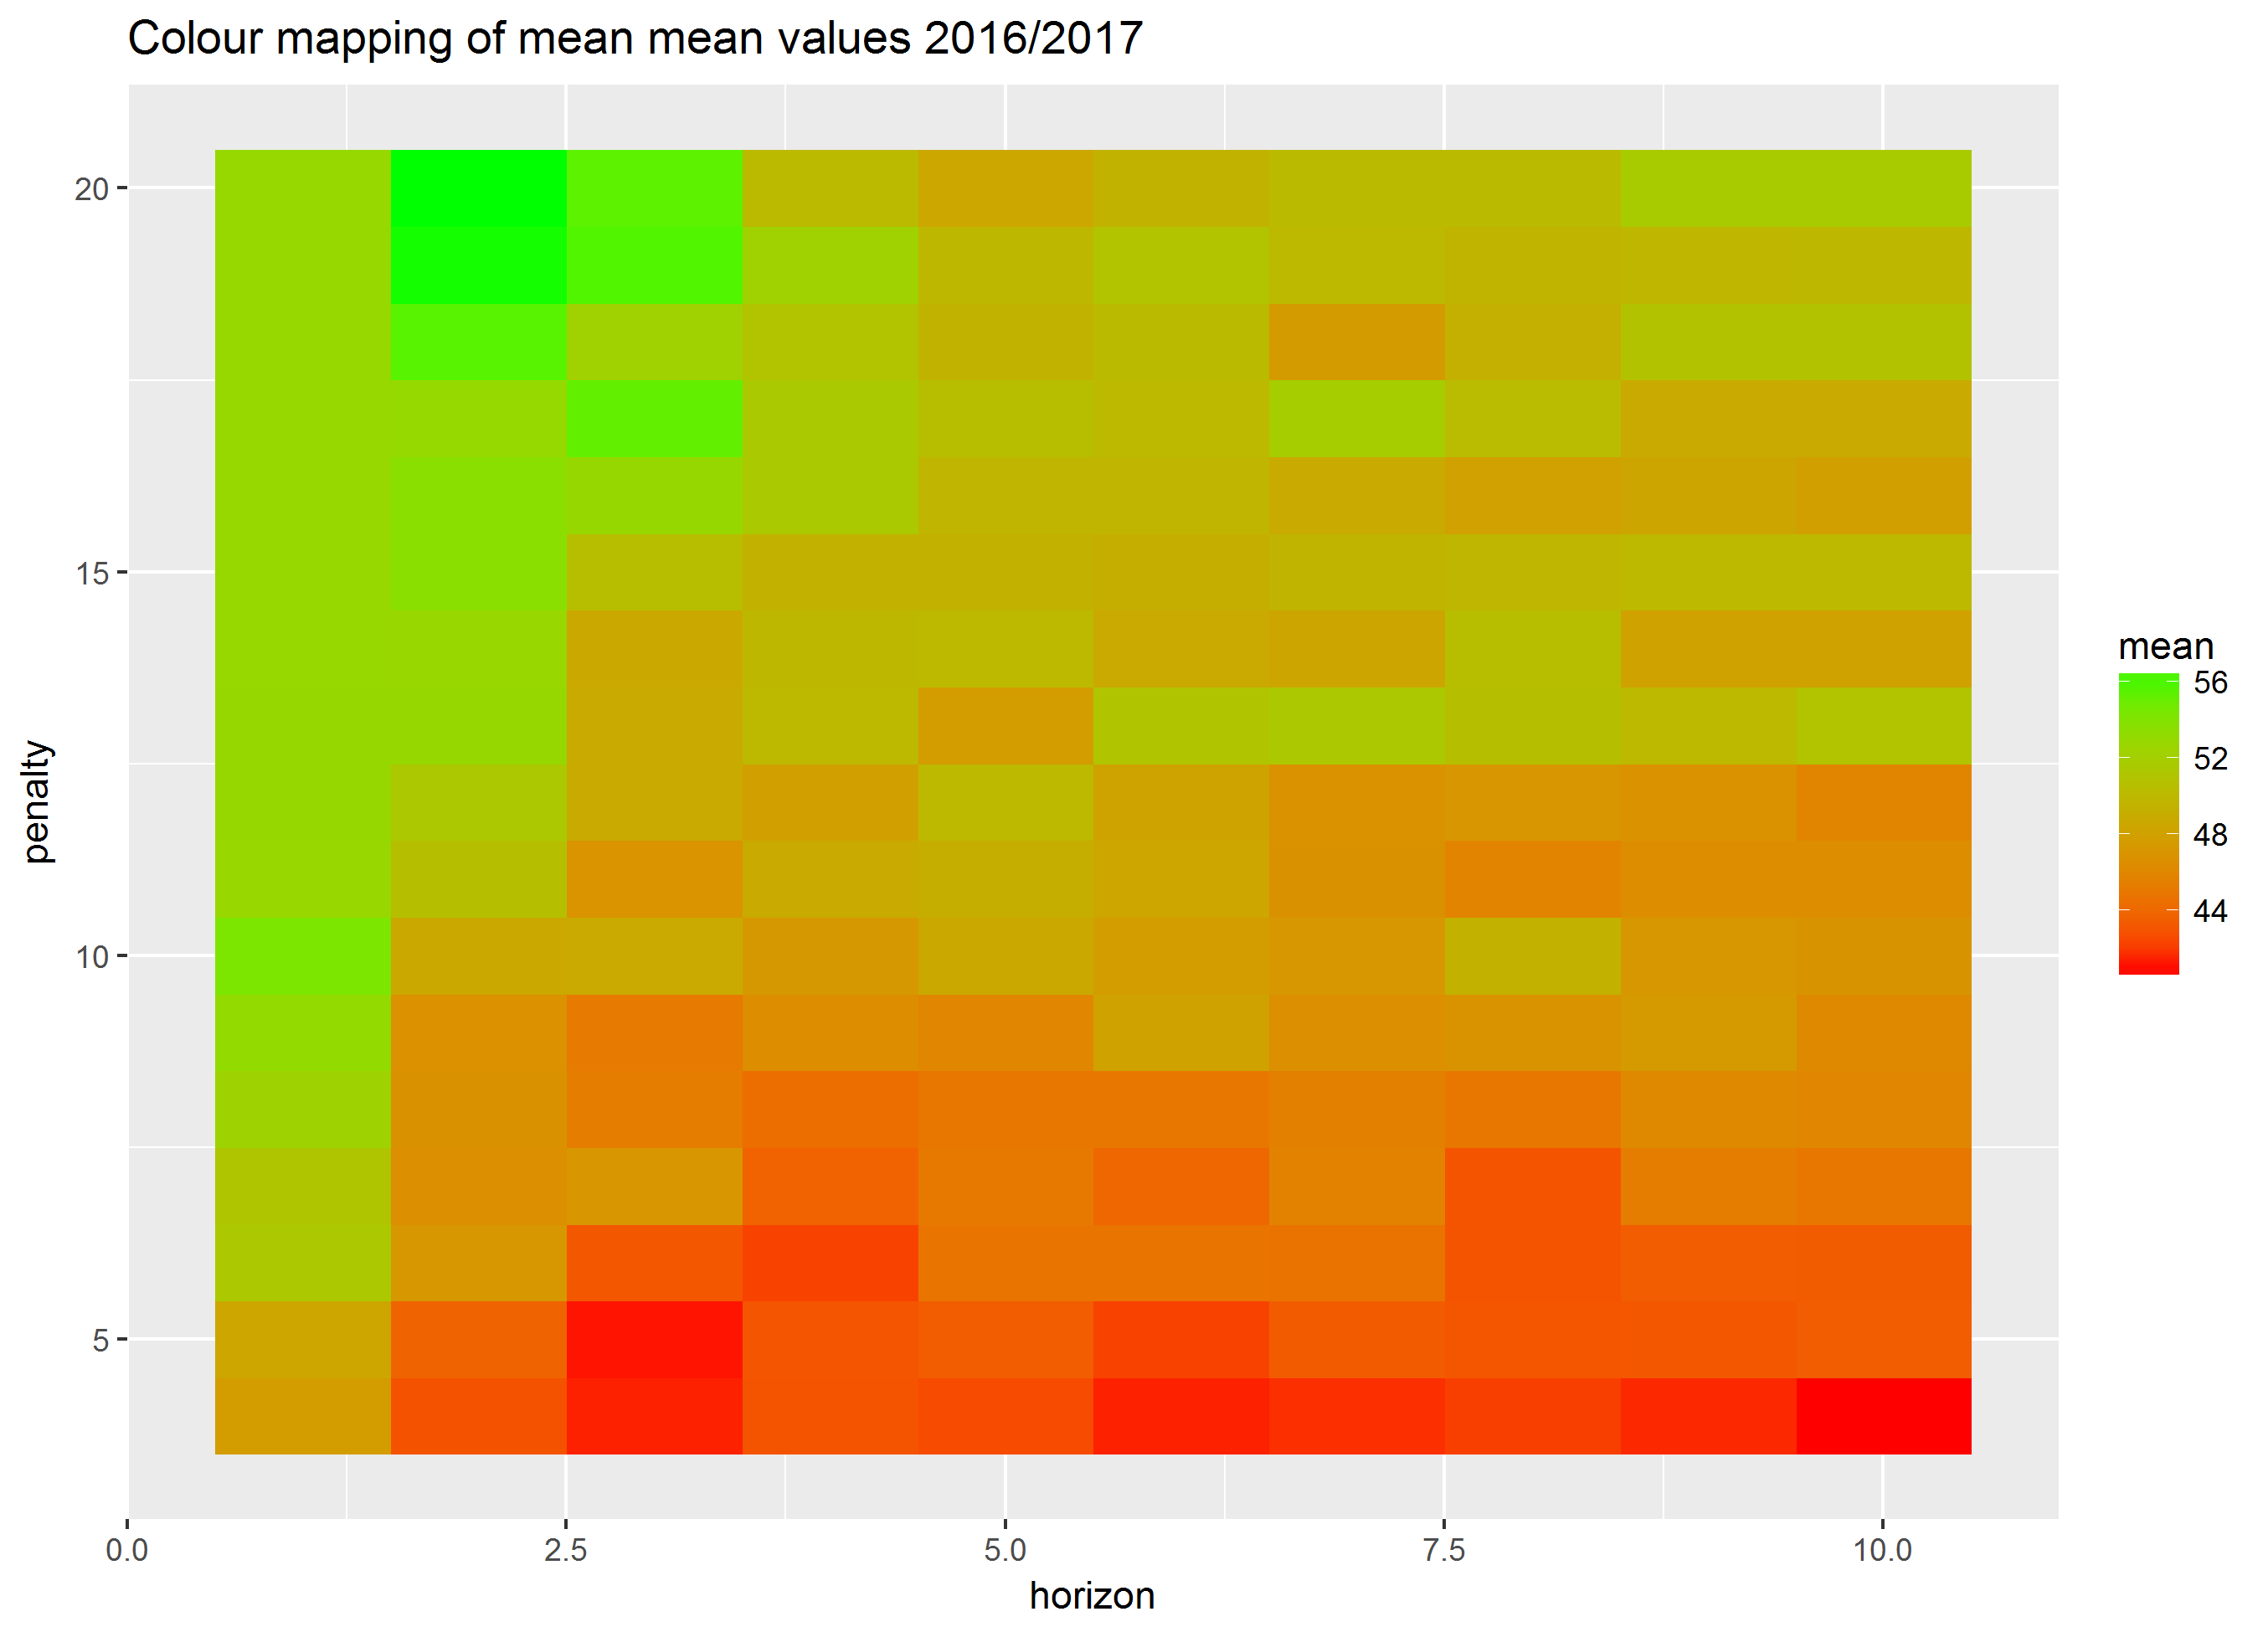
\includegraphics[scale=0.50]{fig/chapter_5/pen_hor_scale.png}
    \caption{The plot shows how the mean value of the entire 2016/2017 season changes depending on horizon and penalty term}
\end{figure}











